\chapter{Planten om ons heen}\label{ch:g1:plants-around-us}

Een madeliefje in het gazon, mos op de muur, de grote kastanjeboom op
het schoolplein: geen van alle zal ooit weglopen, en toch leven ze
allemaal. \omterm{def:g1:plants-around-us:plant}{Planten} zijn de stille levende wezens --- ze worden geboren,
ze eten, ze groeien, soms honderden jaren lang, en dat allemaal zonder
van hun plek te komen.

\section{Planten zijn levende wezens}

\begin{definition}[Plant]\label{def:g1:plants-around-us:plant}
Een \emph{plant}\index{plant} is een \omterm{def:g1:living-or-not:living}{levend wezen} dat vast in de grond
staat en zijn eigen voedsel maakt met behulp van licht. Gras,
madeliefjes, tomatenplanten en bomen zijn allemaal planten. De meeste
planten zijn groen.
\end{definition}

\begin{example}[Het madeliefje leeft]\label{ex:g1:plants-around-us:daisy}
Loop de kenmerken van leven na bij een madeliefje: het is uit een
zaadje geboren; het eet --- water uit de grond en licht uit de lucht;
het groeit; het maakt zaadjes waaruit nieuwe madeliefjes komen; het
gaat dood in de vorst. Alle kenmerken zijn er. Het madeliefje leeft
net zo goed als de kat --- het is er alleen veel stiller over.
\end{example}

\begin{omfigure}
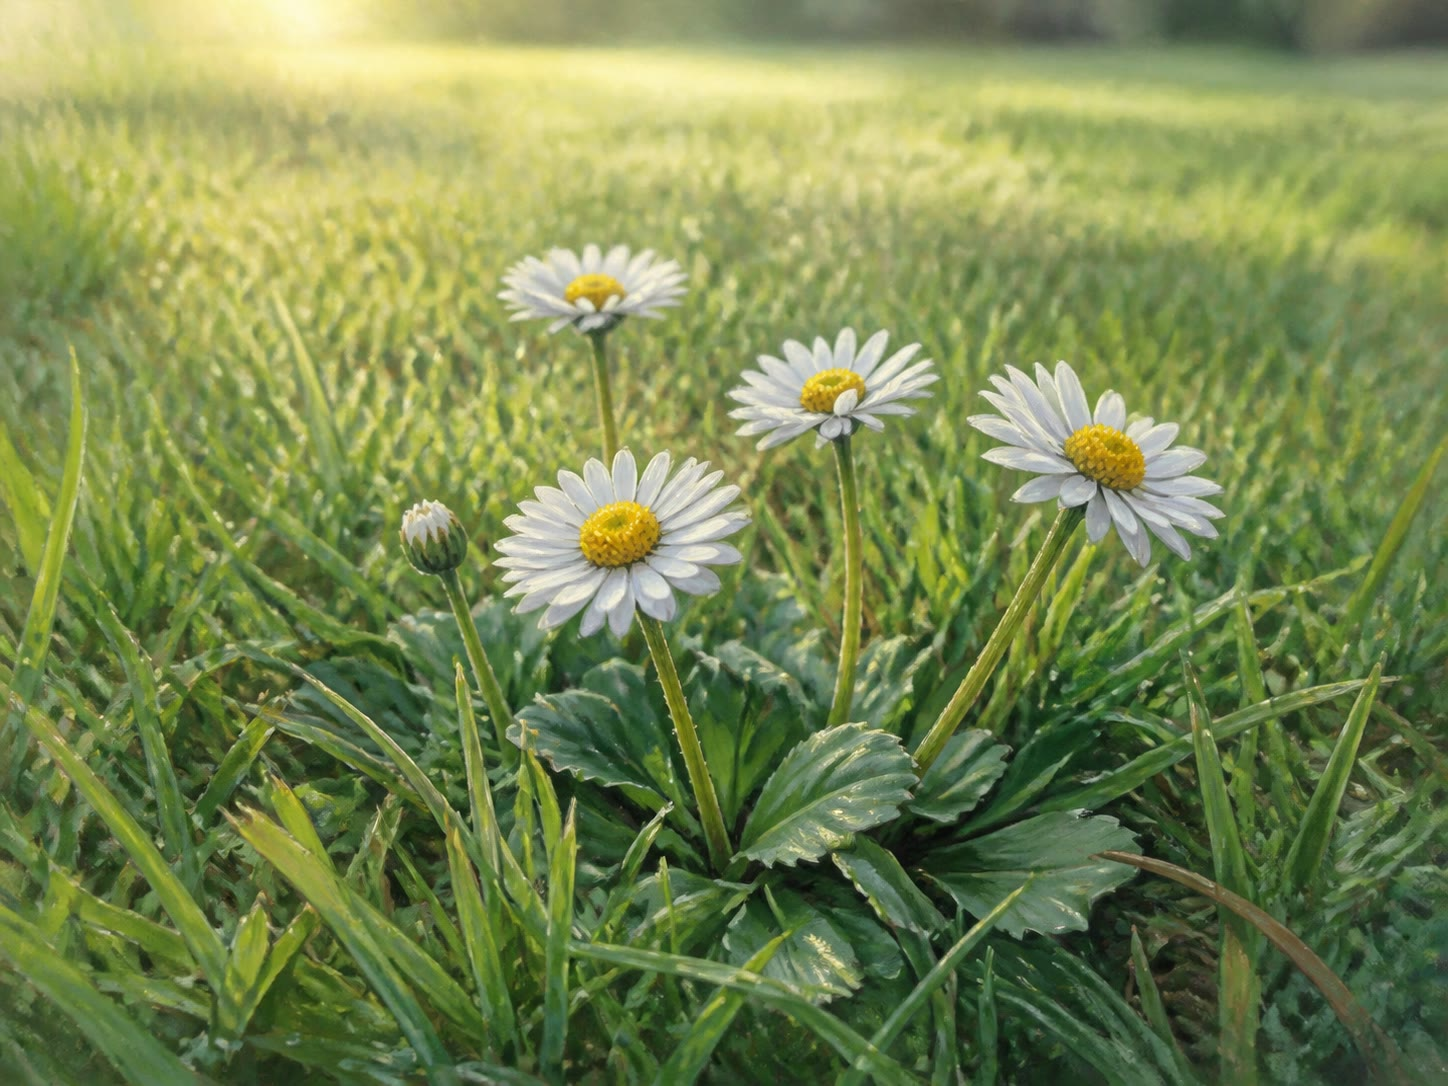
\includegraphics[width=0.58\linewidth]{images/book1/ai/g1-plants-daisy.jpg}

{\small Madeliefjes in het gazon: uit zaadjes geboren, etend van licht
en water, in alle stilte levend.}
\end{omfigure}

\begin{remark}[Levend zonder te rennen]\label{rem:g1:plants-around-us:still}
\omterm{def:g1:plants-around-us:plant}{Planten} lopen niet, maar ze staan ook niet helemaal stil. Een
zonnebloem draait overdag mee met het licht, en een \omterm{def:g1:plants-around-us:plant}{plant} op de
vensterbank buigt langzaam naar het raam toe. \omterm{def:g1:plants-around-us:plant}{Planten} bewegen door te
\emph{groeien} --- te langzaam voor onze ogen, snel genoeg voor een
week kijken.
\end{remark}

\section{De delen van een plant}

\begin{definition}[Delen van een plant]\label{def:g1:plants-around-us:parts}
Een bloeiende \omterm{def:g1:plants-around-us:plant}{plant} heeft vier hoofddelen:
\begin{enumerate}
  \item de \emph{wortels}\index{wortel}, verborgen in de grond, die de
        \omterm{def:g1:plants-around-us:plant}{plant} op zijn plaats houden en water drinken;
  \item de \emph{stengel}\index{stengel}, die de \omterm{def:g1:plants-around-us:plant}{plant} rechtop zet en
        water naar de bladeren brengt;
  \item de \emph{bladeren}\index{blad}, plat en groen, die het licht
        opvangen;
  \item de \emph{bloem}\index{bloem}, die de zaden zal maken.
\end{enumerate}
\end{definition}

\begin{omfigure}
\begin{tikzpicture}
  \node[anchor=south west, inner sep=0] (img) at (0,0)
    {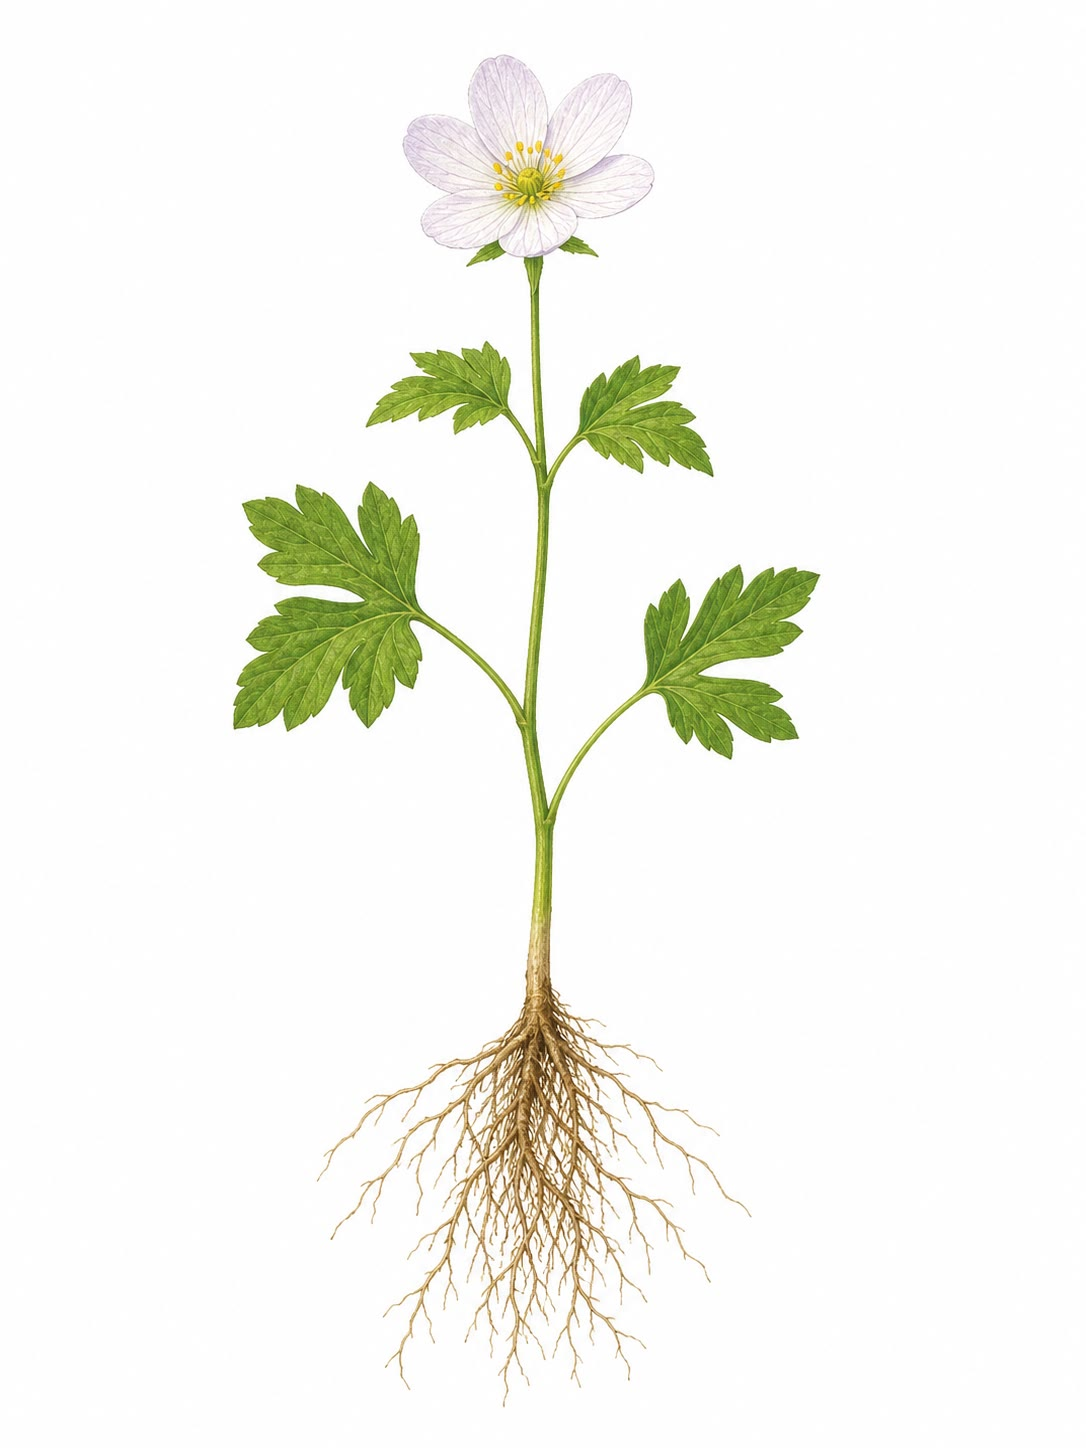
\includegraphics[width=0.5\linewidth]{images/book1/ai/fig-plant-uprooted.jpg}};
  \begin{scope}[x={(img.south east)}, y={(img.north west)},
      every node/.style={font=\small}]
    \draw[omDef, thick] (0.55,0.91) -- (0.74,0.93) node[right] {bloem};
    \draw[omDef, thick] (0.68,0.57) -- (0.84,0.62) node[right] {blad};
    \draw[omDef, thick] (0.51,0.33) -- (0.74,0.36) node[right] {stengel};
    \draw[omDef, thick] (0.58,0.13) -- (0.78,0.16) node[right] {wortels};
  \end{scope}
\end{tikzpicture}

{\small De vier delen van een bloeiende \omterm{def:g1:plants-around-us:plant}{plant}, in hun geheel uit de
grond getrokken: in de bodem doen de \omterm{def:g1:plants-around-us:parts}{wortels} hun werk onzichtbaar,
onder de aarde.}
\end{omfigure}

\begin{example}[Een onkruidje uittrekken]\label{ex:g1:plants-around-us:weed}
Trek voorzichtig een onkruidje uit losse, natte aarde en je haalt het
verborgen deel omhoog: een pluk bleke \omterm{def:g1:plants-around-us:parts}{wortels}, soms langer dan de hele
groene \omterm{def:g1:plants-around-us:plant}{plant} erboven. Nu kun je de \omterm{def:g1:plants-around-us:plant}{plant} van onder naar boven lezen:
\omterm{def:g1:plants-around-us:parts}{wortels}, \omterm{def:g1:plants-around-us:parts}{stengel}, \omterm{def:g1:plants-around-us:parts}{bladeren} --- en, met geluk, een \omterm{def:g1:plants-around-us:parts}{bloem}.
\end{example}

\begin{definition}[Boom]\label{def:g1:plants-around-us:tree}
Een \emph{boom}\index{boom} is een grote \omterm{def:g1:plants-around-us:plant}{plant} waarvan de \omterm{def:g1:plants-around-us:parts}{stengel} van
hout is. De houtige \omterm{def:g1:plants-around-us:parts}{stengel} van de boom heet de
\emph{stam}\index{stam}; die splitst zich in \emph{takken}\index{tak},
die de \omterm{def:g1:plants-around-us:parts}{bladeren} dragen.
\end{definition}

\begin{example}[De kastanjeboom]\label{ex:g1:plants-around-us:tree}
De kastanjeboom op het plein heeft hetzelfde bouwplan als het
madeliefje, maar dan groter en harder: \omterm{def:g1:plants-around-us:parts}{wortels} onder de grond, een stam
in plaats van een zachte \omterm{def:g1:plants-around-us:parts}{stengel}, takken met duizenden \omterm{def:g1:plants-around-us:parts}{bladeren}, en in
de lente \omterm{def:g1:plants-around-us:parts}{bloemen}. Het madeliefje leeft één jaar; de kastanjeboom kan
langer dan honderd jaar leven.
\end{example}

\section{Wat een plant nodig heeft}

\begin{proposition}[De behoeften van een plant]\label{prop:g1:plants-around-us:needs}
Om te leven en te groeien heeft een \omterm{def:g1:plants-around-us:plant}{plant} \emph{water}, \emph{licht} en
een plaats voor haar \omterm{def:g1:plants-around-us:parts}{wortels} nodig, meestal \emph{aarde}\index{aarde}.
Een \omterm{def:g1:plants-around-us:plant}{plant} die in het donker staat, of die nooit water krijgt, verwelkt
en gaat dood.
\end{proposition}
\admitted

\begin{example}[De vergeten plant]\label{ex:g1:plants-around-us:wilt}
Vergeet de klasplant water te geven voor de vakantie: haar \omterm{def:g1:plants-around-us:parts}{bladeren}
hangen slap en zielig omlaag --- ze verwelkt. Geef haar water, en een
paar uur later staan de \omterm{def:g1:plants-around-us:parts}{bladeren} weer rechtop. Water was wat ontbrak.
\end{example}

\begin{method}[Voor een plant zorgen]\label{met:g1:plants-around-us:care}
\begin{enumerate}
  \item Zet de pot waar daglicht bij kan;
  \item geef de aarde water als die droog aanvoelt --- niet elk uur, de
        \omterm{def:g1:plants-around-us:parts}{wortels} hebben ook lucht nodig;
  \item trek de \omterm{def:g1:plants-around-us:parts}{bladeren} er niet af: dat zijn de lichtvangers van de
        \omterm{def:g1:plants-around-us:plant}{plant};
  \item heb geduld: een \omterm{def:g1:plants-around-us:plant}{plant} antwoordt in dagen, niet in minuten.
\end{enumerate}
\end{method}

\begin{remark}[Planten voeden iedereen]\label{rem:g1:plants-around-us:food}
\omterm{def:g1:plants-around-us:plant}{Planten} zijn belangrijk voor elk \omterm{def:g1:animals-around-us:animal}{dier}. De slak eet de sla, de merel eet
bessen, wij eten brood van tarwe --- een \omterm{def:g1:plants-around-us:plant}{plant}. Zelfs de kat, die geen
sla eet, eet \omterm{def:g1:animals-around-us:animal}{dieren} die \omterm{def:g1:plants-around-us:plant}{planten} gegeten hebben. Zonder \omterm{def:g1:plants-around-us:plant}{planten} zou
niemand anders iets te eten hebben; een later hoofdstuk volgt deze
voedselketens.
\end{remark}

\section{Oefeningen}

\begin{exercise}[$\star$]\label{exo:g1:plants-around-us:1}
Noem de vier delen van een bloeiende \omterm{def:g1:plants-around-us:plant}{plant}, van onder de grond tot
bovenaan.
\end{exercise}

\begin{exercise}[$\star$]\label{exo:g1:plants-around-us:2}
Welk deel van de \omterm{def:g1:plants-around-us:plant}{plant}: (a) drinkt water uit de grond? (b) vangt het
licht op? (c) zal de zaden maken? (d) houdt de \omterm{def:g1:plants-around-us:plant}{plant} rechtop?
\end{exercise}

\begin{exercise}[$\star$]\label{exo:g1:plants-around-us:3}
Het madeliefje loopt nooit. Loop de kenmerken van leven na en zeg
waarom het toch een \omterm{def:g1:living-or-not:living}{levend wezen} is.
\end{exercise}

\begin{exercise}[$\star$]\label{exo:g1:plants-around-us:4}
Wat zijn de bijzondere namen van de \omterm{def:g1:plants-around-us:parts}{stengel} van de \omterm{def:g1:plants-around-us:tree}{boom} en van de delen
die zijn \omterm{def:g1:plants-around-us:parts}{bladeren} dragen?
\end{exercise}

\begin{exercise}[$\star$]\label{exo:g1:plants-around-us:5}
Geef de drie dingen die een \omterm{def:g1:plants-around-us:plant}{plant} nodig heeft om te leven, uit
\cref{prop:g1:plants-around-us:needs}.
\end{exercise}

\begin{exercise}[$\star$]\label{exo:g1:plants-around-us:6}
De klasplant heeft slappe, hangende \omterm{def:g1:plants-around-us:parts}{bladeren}. Wat is er waarschijnlijk
vergeten? Wat gebeurt er nadat het gegeven is?
\end{exercise}

\begin{exercise}[$\star$]\label{exo:g1:plants-around-us:7}
In welke opzichten zijn het madeliefje en de kastanjeboom hetzelfde? In
welke twee opzichten verschillen ze?
\end{exercise}

\begin{exercise}[$\star$]\label{exo:g1:plants-around-us:8}
Probeer het: zet één boonplantje (of een bakje tuinkers) bij het raam
en één in een donkere kast, en geef ze allebei water. Kijk na een week.
Welk verschil verwacht je, en welke behoefte verklaart dat?
\end{exercise}

\begin{exercise}[$\star\star$]\label{exo:g1:plants-around-us:9}
Leo zegt: ``\omterm{def:g1:plants-around-us:plant}{Planten} leven niet echt --- ze doen nooit iets.'' Geef hem
twee dingen die een \omterm{def:g1:plants-around-us:plant}{plant} wél doet, langzaam maar zeker, uit
\cref{rem:g1:plants-around-us:still} en
\cref{ex:g1:plants-around-us:daisy}.
\end{exercise}

\begin{exercise}[$\star\star$]\label{exo:g1:plants-around-us:10}
Een \omterm{def:g1:plants-around-us:parts}{wortel} is oranje en groeit onder de grond. Welk deel van de
wortelplant eten we, denk je, als je naar de figuur van de plantendelen
kijkt? Welke aanwijzing geeft ``onder de grond''?
\end{exercise}
